\section{Results}\label{sec:results}
The controllers have been implemented and tested in the real quadcopter. The real results for the attitude controller and simulation results with the network and the model simulated in MATLAB Simulink for the translational controllers are presented. 

The obtained model parameters can be seen in \autoref{ParametersQuadcopter}. 
\begin{table}[H]
    \centering
    \begin{tabular}{c|c|c}
        %------------------------------------------------------------------------------------------
        \textbf{Symbol} &\textbf{Value} &\textbf{Units}\\
        \hline %-----------------------------------------------------------------------------------
        $m$ & 0.996       &kg\\
        \hline %-----------------------------------------------------------------------------------
        $L$  &   0.225       & m\\
        \hline %-----------------------------------------------------------------------------------
        $J_x$  & 0.01073       & \si{kg \  m^2}\\
        \hline %-----------------------------------------------------------------------------------
        $J_y$  & 0.01073       & \si{kg \  m^2}\\
        \hline %-----------------------------------------------------------------------------------
        $J_z$  & 0.02135       & \si{kg \  m^2}\\
        \hline %-----------------------------------------------------------------------------------
        $k_{\mathrm{th}}$  & $1.32922\cdot10^{-5}$       & \si{N s^2 rad^{-2}}\\
        \hline %-----------------------------------------------------------------------------------
        $k_{\mathrm{d}}$  & $9.39741 \cdot10^{-7}$       & \si{N m s^2  rad^{-2}}\\
        \hline %-----------------------------------------------------------------------------------
        $\overline{\omega}_i$& 429      & \si{rad \ s^{-1}}\\
        
    \end{tabular}
    \caption{Parameters used though the analysis and design.}
    \label{ParametersQuadcopter}
\end{table}
The mass and the length have been measured, $k_{\mathrm{th}}$ and $k_{\mathrm{d}}$ have been obtained through testing the propellers when rotating at different speeds and the moments of inertia have been calculated analytically considering the quadcopter as a combination of different masses with known moment of inertia.

The value of delay used in the simulation \fxnote{WRITE NUMBER} milliseconds and the packet loss probability is set to zero.

The attitude controller is defined by the designed $\vec{Q}$ and $\vec{R}$ diagonal matrices shown below and the chosen observer poles, which are $[-11, -12, -13]$.
%\footnotesize{
%\begin{flalign}   \label{Fematrix}
%	\vec{F}&=
%	\begin{bmatrix}
%		 0.00    & -165.15 & -223.35  &  0.00   &-44.04 & -68.52  \ \ \ \\
%		 165.15  &  0.00   & 223.35   &  44.04  & 0.00  &  68.52  \ \ \ \\
%		 0.00    & 165.15  & -223.35  &  0.00   &44.04  & -68.52  \ \ \ \\
%		 -165.15 & 0.00    & 223.35   & -44.04  & 0.00  &  68.52  \ \ \ 
%	\end{bmatrix}\nonumber\\
%		\vec{F}_{\mathrm{int}}&=
%		\begin{bmatrix}
%		   0.00   & -220.97 & -250.00  \ \ \ \\
%		   220.97 &   0.00  & 250.00   \ \ \ \\
%		   0.00   & 220.97  & -250.00  \ \ \ \\
%		  -220.97 &  0.00   &  250.00  \ \ \ 
%		\end{bmatrix}\nonumber
%\end{flalign}}
%\normalsize
\begin{center}
\noindent$\vec{Q}=diag\left(\frac{1}{0.2^2},\frac{1}{0.2^2},\frac{1}{0.1^2},\frac{1}{0.5^2},\frac{1}{0.5^2},\frac{1}{0.3^2},\frac{1}{0.08^2},\frac{1}{0.08^2},\frac{1}{0.05^2}\right)$

\noindent$\vec{R}=diag\left(\frac{1}{25^2},\frac{1}{25^2},\frac{1}{25^2},\frac{1}{25^2}\right) $
\end{center}

The  controllers for $\dot{x}_{\mathrm{I}}$, $\dot{y}_{\mathrm{I}}$, $\dot{z}_{\mathrm{I}}$, $x_{\mathrm{I}}$, $y_{\mathrm{I}}$ and $z_{\mathrm{I}}$ are
\begin{minipage}{0.45\linewidth}
	\begin{flalign}
		C_{\dot{x}_{\mathrm{I}}}=-C_{\dot{y}_{\mathrm{I}}}=-0.0038\frac{1+20s}{s},\nonumber
	\end{flalign}
\end{minipage}   \hfill 
\begin{minipage}{0.45\linewidth}
	\begin{flalign}
		C_{\dot{z}_{\mathrm{I}}}=-201.8\frac{s+0.8}{s}\ ,\nonumber
	\end{flalign}
\end{minipage}\\

\begin{minipage}{0.45\linewidth}
	\begin{flalign}
		C_{x_{\mathrm{I}}}=C_{y_{\mathrm{I}}}=0.3,\nonumber
	\end{flalign}
\end{minipage}   \hfill 
\begin{minipage}{0.45\linewidth}
	\begin{flalign}
		C_{z_{\mathrm{I}}}=1\ .\nonumber
	\end{flalign}
\end{minipage}\\

These controllers are discretized using the Tustin method with a sampling frequency of 28 Hz. This is the fastest available frequency in which data can be acquired from the motion tracking system, transmitted to the quadcopter and read by the microcontroller.

\autoref{fig:rollref} and \ref{fig:pitchref} show the attitude controller response when tracking a reference in pitch angle.
\begin{figure}[H]
	\centering
	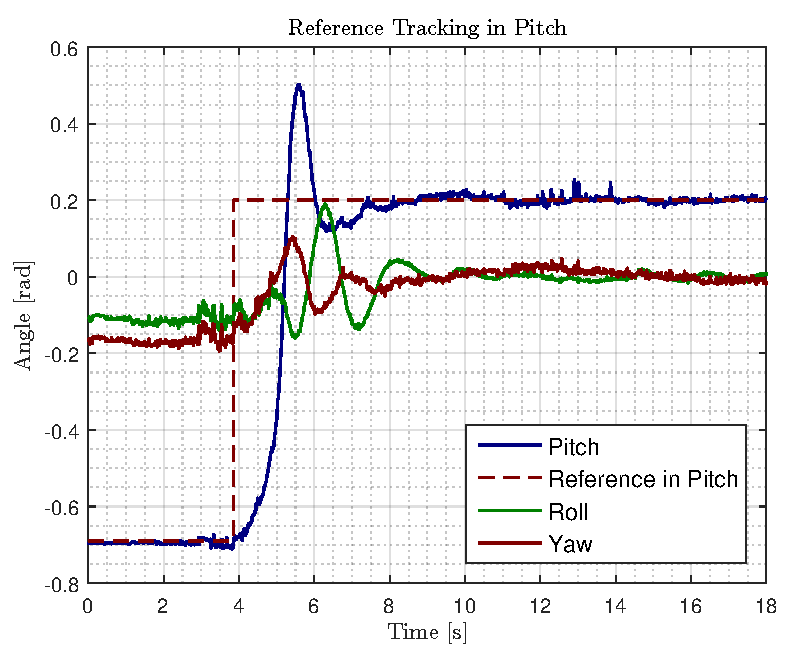
\includegraphics[width=.4\textwidth]{figures/pitchRefAcceptAllAngles}
	\caption{Real attitude control response when tracking a reference in pitch.}
	\label{fig:pitchref}
\end{figure}

In \autoref{fig:positionControl}, the simulated step responses of the translational controllers along the three axes are depicted.
\begin{figure}[H]
	\centering
	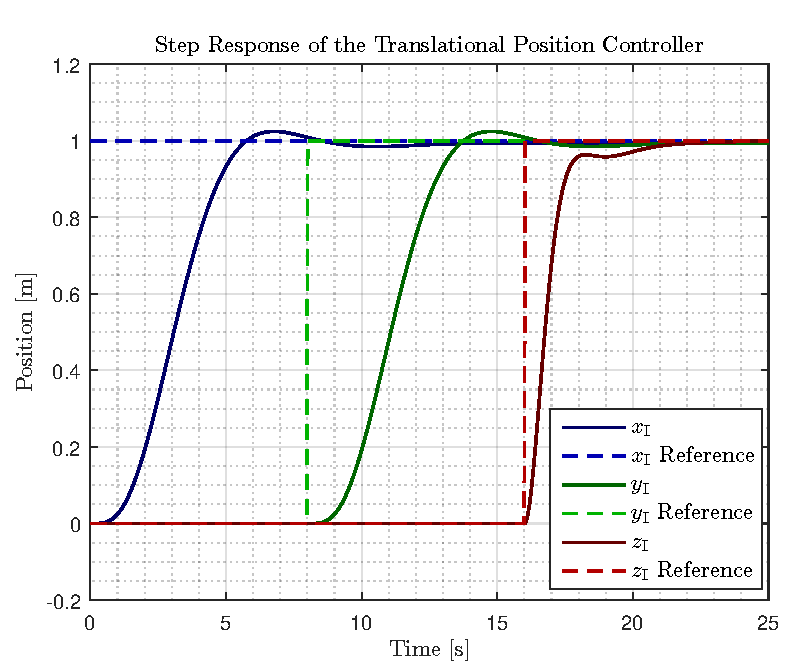
\includegraphics[width=.4\textwidth]{figures/stepTrans}
	\caption{Position control results in the three inertial axes directions. The references given to the control system are shown with dashed lines.}
	\label{positionControl}
\end{figure}
%
%The inner attitude controller results are also included and shown in \autoref{AttitudeControl} so the performance of the attitude control can be evaluated. 
%\begin{figure}[H]
%	\centering
%	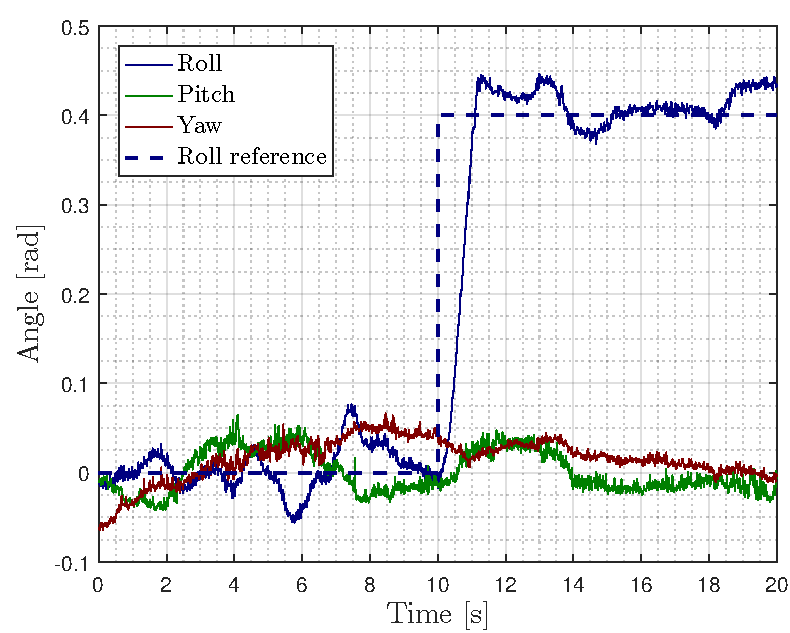
\includegraphics[width=.4\textwidth]{figures/AttitudeControl}
%	\caption{Attitude control results in the three angles. The references given to the attitude control system are shown with dashed lines.}
%	\label{AttitudeControl}
%\end{figure}